	\subsection{Task Assigned}
		For the EE4H Computer Vision assignment the task set is to examine images of classic playing cards and develop an automated software solution for classifying their suit and rank without human intervention. To do this, an understanding of the existing techniques available to use must be gained, a software solution developed that meets the task requirements and that software must be evaluated and tested to ensure it is working correctly. 

		Therefore the task can be split into the following stages:

		\begin{enumerate}
			\item Image pre-processing to enhance features.
			\item Card isolation from input image.
			\item For each card:
			\begin{enumerate}
				\item Correct perspective
				\item Correct rotation
				\item Isolate suit symbol and rank symbol
				\item Find card rank (numerical value and picture card rank)
				\item Find card suit using suit symbol
			\end{enumerate}
			\item Display results of classification to user in easy to understand forms.
		\end{enumerate}

		In doing this the software must be able to compensate for issues that may hinder classification such as uneven lighting, different card orientations, single and multiple card images and card reflectivity.
	\subsection{Method Used}
		The chosen method to classify playing cards was determined after the review of literature and is as follows:
		\begin{itemize}
			\item Perform pre-processing to compensate for lighting.
			\item Isolate cards using their stark contours against the background.
			\item Correct isolated card perspective using a Perspective Transform.
			\item Correct card's rotation using corner intensities.
			\item Remove white background from card and use redness in corners to determine suit colour.
			\item Isolate rank symbol and suit symbol areas from isolated card corners.
			\item Use blob counting after morphological erosion and closing to determine rank in the case of value cards (2 -- 10), and morphological Hit-or-Miss in the case of picture cards.
			\item Present output classifications as a GUI cascade and system console textual output.
		\end{itemize}

		This method involves both high and low level computer vision and mathematical morphological techniques that are detailed in the Review section \secref{sec:review} before implementation as documented in the Implementation section \secref{sec:implementation}. Using this series of stages the software is able to compensate for many of the issues highlighted in the last section. However, it is designed for the classical playing card style, used the world over, and not for overly stylised, custom, heavily themed or obfuscated decks.
	% TODO: Is this a good heading?
	\subsection{Findings}
		% TODO: Figure with a capital F?
		After successful implementation of the above stages (and techniques employed therein) the software is able to correctly isolate [TODO: How successful?] cards in moderately favourable conditions. The software is also able to isolate and correctly transform cards at many orientations relative to the camera as well as discard playing cards that are face down. Once these cards have been isolated, each card's rank and symbol are correctly identified with a high rate of success [TODO: How high?]. This is illustrated in Figure~\ref{fig:success} below:

		\begin{figure}[H]
			\centering
			\begin{subfigure}[b]{\textwidth}
				\centering
				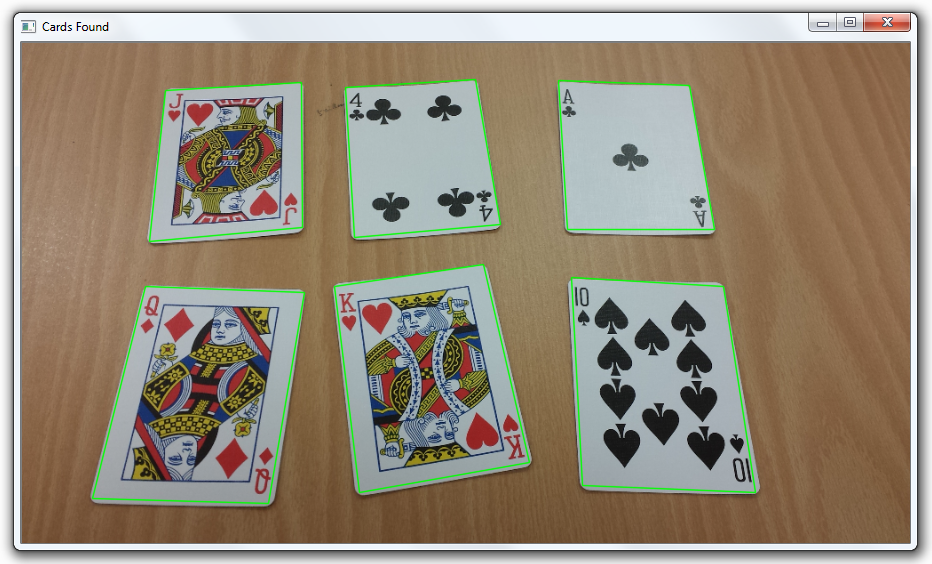
\includegraphics[width=0.8\textwidth]{chris/image1}
				\caption{}
			\end{subfigure}
		\end{figure}
		\begin{figure}[H]
			\ContinuedFloat
			\centering
			\begin{subfigure}[b]{\textwidth}
				\centering
				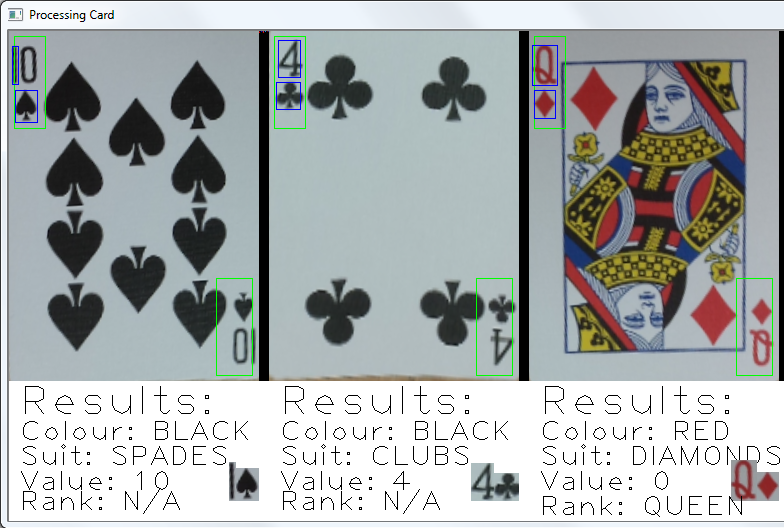
\includegraphics[width=0.8\textwidth]{chris/image2}
				\caption{}
			\end{subfigure}
		\end{figure}
		\begin{figure}[H]
			\ContinuedFloat
			\centering
			\begin{subfigure}[b]{\textwidth}
				\centering
				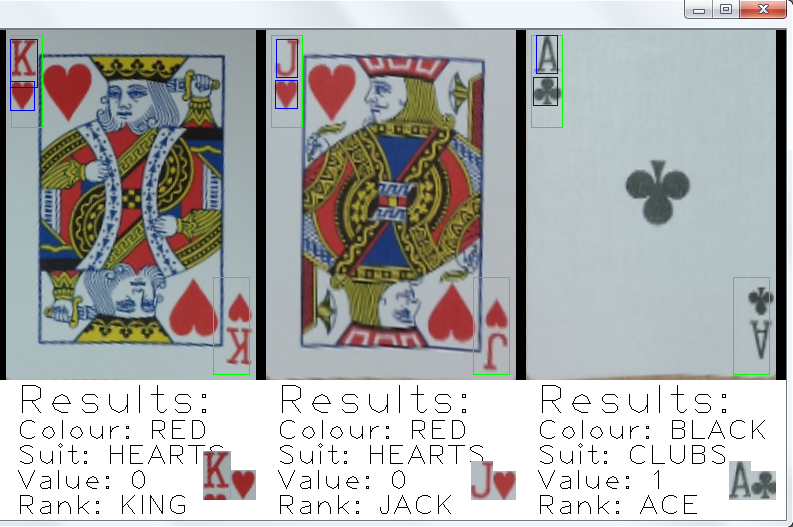
\includegraphics[width=0.8\textwidth]{chris/image3}
				\caption{}
			\end{subfigure}
			\caption{A set of playing cards (a) at various orientations with a visual output of successful classifications (b) (c)}
			\label{fig:success}
		\end{figure}

		However, when the input image is of low quality or there are too many cards per image (\textgreater $\approx$12) the classification is not always successful, but it has been found that in these situations is at least a small number are correctly identified, particularly if the unfavourable light varies across the image. Some examples of such situations are shown in Figure~\ref{fig:fail}:

		% TODO: Images with window borders from now on
		% TODO: Light distortion still an issue?
		\begin{figure}[H]
			\centering
			\begin{subfigure}[b]{\textwidth}
				\centering
				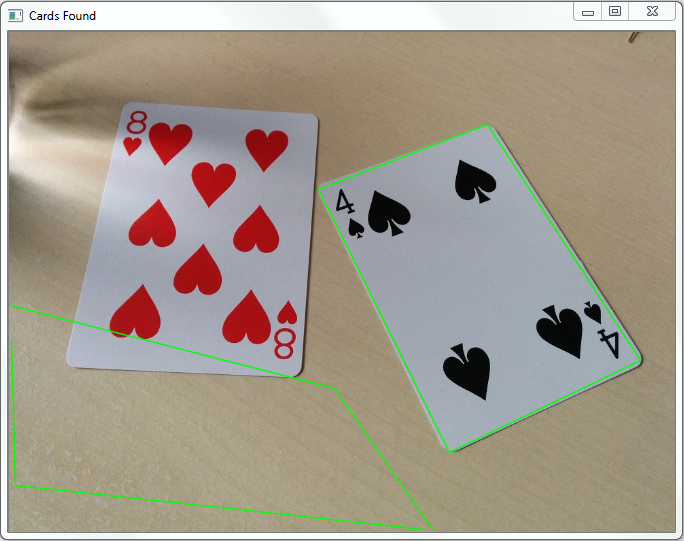
\includegraphics[width=0.8\textwidth]{chris/image4}
				\caption{}
			\end{subfigure}
		\end{figure}
		\begin{figure}[H]
			\ContinuedFloat
			\centering
			\begin{subfigure}[b]{\textwidth}
				\centering
				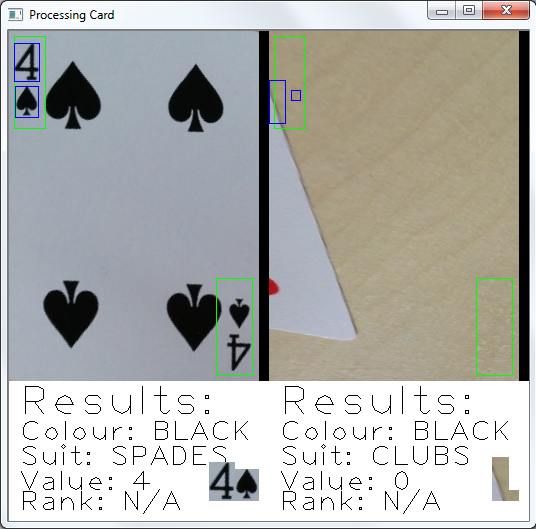
\includegraphics[width=0.8\textwidth]{chris/image5}
				\caption{}
			\end{subfigure}
			\caption{An example of miss-classification (b) due to significant lighting distortion (a)}
			\label{fig:fail}
		\end{figure}